\documentclass[xga]{xdvislides}
\usepackage[landscape]{geometry}
\usepackage{graphics}
\usepackage{graphicx}
\usepackage{colordvi}

\begin{document}
\setfontphv

%%% Headers and footers
\lhead{\slidetitle}                               % default:\lhead{\slidetitle}
\chead{CS631 - Advanced Programming in the UNIX Environment}% default:\chead{\relax}
\rhead{Slide \thepage}                       % default:\rhead{\sectiontitle}
\lfoot{\Gray{HTTP, Coding Practices}}% default:\lfoot{\slideauthor}
\cfoot{\relax}                               % default:\cfoot{\relax}
\rfoot{\Gray{\today}}

\newcommand{\smallish}{\fontsize{15}{20}\selectfont}

\vspace*{\fill}
\begin{center}
	\Hugesize
		CS631 - Advanced Programming in the UNIX Environment\\ [1em]
		HTTP; Code Reading\\ [1em]
	\hspace*{5mm}\blueline\\ [1em]
	\Normalsize
		Department of Computer Science\\
		Stevens Institute of Technology\\
		Jan Schaumann\\
		\verb+jschauma@stevens.edu+ \\
		\verb+https://stevens.netmeister.org/631/+
\end{center}
\vspace*{\fill}

\subsection{HTTP}
\vspace{.5in}
\begin{center}
	\Huge
	Hypertext Transfer Protocol
	\\
	\vspace{.5in}
	RFC1945 (HTTP/1.0), RFC2616 (HTTP/1.1), RFC7540 (HTTP/2)\\
	\vspace{.5in}
	A simple request/response protocol.
\end{center}
\Normalsize

\subsection{The Hypertext Transfer Protocol}
HTTP is a request/response protocol:
\begin{enumerate}
	\item client sends a request to the server
	\item server responds
\end{enumerate}

\subsection{The Hypertext Transfer Protocol}
HTTP is a request/response protocol:
\begin{enumerate}
	\item client sends a request to the server
		\begin{itemize}
			\item request method
			\item URI
			\item protocol version
			\item request modifiers
			\item client information
		\end{itemize}
	\item server responds
\end{enumerate}

\subsection{HTTP: A client request}
\vspace*{.5in}
\\
\Hugesize
\begin{center}
\begin{verbatim}
$ telnet www.google.com 80
Trying 173.194.75.147...
Connected to www.google.com.
Escape character is '^]'.
GET / HTTP/1.0
\end{verbatim}
\end{center}
\Normalsize
\vspace*{\fill}


\subsection{The Hypertext Transfer Protocol}
HTTP is a request/response protocol:
\begin{enumerate}
	\item client sends a request to the server
		\begin{itemize}
			\item request method
			\item URI
			\item protocol version
			\item request modifiers
			\item client information
		\end{itemize}
	\item server responds
		\begin{itemize}
			\item status line (including success or error code)
			\item server information
			\item entity metainformation
			\item content
		\end{itemize}
\end{enumerate}

\subsection{HTTP: a server response}
%\smallish
\begin{verbatim}
HTTP/1.0 200 OK
Date: Mon, 05 Nov 2018 02:52:21 GMT
Content-Type: text/html; charset=ISO-8859-1
Server: gws
X-XSS-Protection: 1; mode=block
X-Frame-Options: SAMEORIGIN
Set-Cookie: 1P_JAR=2018-11-05-02; expires=Wed, 05-Dec-2018 02:52:21 GMT; path=/; domain=.google.com
Set-Cookie: NID=144=XovVYlBCcjaIYkyum0C3F_7jB7J8jpvabZR_0-ORyWqhmEflAcNKrVdhS0TO144bPrp8qZ3OEYXJw5jmJ_S7Zo3wvu7opk-vY3jZHqCdVscJFnKbmXoH9K6OaNY_b0oVosSZbrXc0ZAdA73dGqr8I-yt4rLCtT5ieEaifVGe7ls;

<!doctype html><html itemscope="itemscope" itemtype="http://schema.org/WebPage">
<head><meta content="Search the...
\end{verbatim}
%\Normalsize

\subsection{The Hypertext Transfer Protocol}
Server status codes:
\begin{itemize}
	\item {\bf 1xx} -- Informational; Request received, continuing process
	\item {\bf 2xx} -- Success; The action was successfully received,
        understood, and accepted
	\item {\bf 3xx} -- Redirection; Further action must be taken in order to
        complete the request
	\item {\bf 4xx} -- Client Error; The request contains bad syntax or
		cannot be fulfilled
	\item {\bf 5xx} -- Server Error; The server failed to fulfill an
		apparently valid request
\end{itemize}

\subsection{HTTP: A client request}
\smallish
\begin{verbatim}
$ telnet www.cs.stevens.edu 80
Trying 155.246.89.84...
Connected to www.cs.stevens-tech.edu.
Escape character is '^]'.
GET / HTTP/1.0

HTTP/1.1 301 Moved Permanently
Date: Mon, 05 Nov 2018 03:20:31 GMT
Server: Apache
Location: https://www.cs.stevens.edu/
Content-Length: 235
Connection: close
Content-Type: text/html; charset=iso-8859-1

<!DOCTYPE HTML PUBLIC "-//IETF//DTD HTML 2.0//EN">
<html><head>
\end{verbatim}
\Normalsize

\subsection{HTTP: A client request}
\smallish
\begin{verbatim}
$ openssl s_client -crlf -servername www.cs.stevens.edu -connect www.cs.stevens.edu:443
[...]
GET / HTTP/1.1
Host: www.cs.stevens.edu

HTTP/1.1 302 Found
Date: Mon, 06 Nov 2017 19:02:10 GMT
Server: Apache
Location: https://www.stevens.edu/ses/cs
Vary: Accept-Encoding
Content-Length: 214
Content-Type: text/html; charset=iso-8859-1

<!DOCTYPE HTML PUBLIC "-//IETF//DTD HTML 2.0//EN">
\end{verbatim}
\Normalsize

\subsection{HTTP: A client request}
\smallish
\begin{verbatim}
$ openssl s_client -crlf -servername www.stevens.edu -connect www.stevens.edu:443
[...]
GET / HTTP/1.1
Host: www.stevens.edu

HTTP/1.1 301 Moved Permanently
Date: Mon, 06 Nov 2017 19:09:21 GMT
Content-Type: text/html; charset=UTF-8
Transfer-Encoding: chunked
Set-Cookie: __cfduid=def9b13568803339571c6eff22b37f43c1509995361;
expires=Tue, 06-Nov-18 19:09:21 GMT; path=/; domain=.stevens.edu; HttpOnly
Last-Modified: Mon, 06 Nov 2017 13:27:15 GMT
Location: https://www.stevens.edu/schaefer-school-engineering-science/departments/computer-science
Via: 1.1 varnish-v4
Server: cloudflare-nginx
Strict-Transport-Security: max-age=15552000
\end{verbatim}
\Normalsize


\subsection{HTTP: A client request}
\smallish
\begin{verbatim}
[...]
GET /schaefer-school-engineering-science/departments/computer-science HTTP/1.1
Host: www.stevens.edu

HTTP/1.1 200 OK
Date: Mon, 06 Nov 2017 19:11:20 GMT
Content-Type: text/html; charset=utf-8
Set-Cookie: __cfduid=dfa773452cb45ba58a5b356568cb3715e1509995480;
expires=Tue, 06-Nov-18 19:11:20 GMT; path=/; domain=.stevens.edu; HttpOnly
Last-Modified: Mon, 06 Nov 2017 15:44:53 GMT
Via: 1.1 varnish-v4
X-Generator: Drupal 7 (http://drupal.org)
X-Varnish: 12117551 14890606
Strict-Transport-Security: max-age=15552000
Server: cloudflare-nginx

<!DOCTYPE html>
<html lang="en" class="no-js">
\end{verbatim}
\Normalsize

\subsection{HTTP: A client request}
\begin{center}
	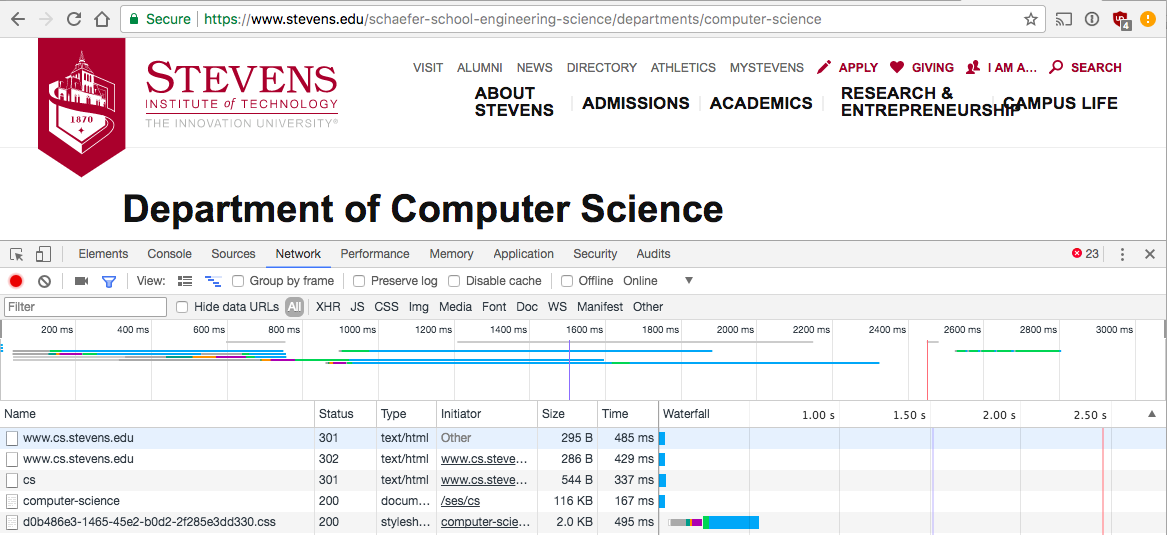
\includegraphics[scale=0.6]{pics/www.cs.stevens.edu.eps}
\end{center}


\subsection{HTTP - more than just text}
HTTP is a {\em Transfer Protocol} -- serving {\em data}, not any specific
text format.

\begin{itemize}
	\item {\tt Accept-Encoding} client header can specify different formats
		such as {\em gzip}, {\em Shared Dictionary Compression over HTTP (SDCH)} etc.
	\item corresponding server headers: {\tt Content-Type} and
		{\tt Content-Encoding}
\end{itemize}
\begin{center}
	
\includegraphics[scale=2.0]{pics/datatransfer.eps}
\end{center}

\subsection{HTTP - more than just static data}
HTTP is a {\em Transfer Protocol} -- what is transferred need not be
static; resources may generate different data to return based on many
variables.

\begin{itemize}
	\item CGI -- resource is {\em executed}, needs to generate
		appropriate response headers
	\item server-side scripting (ASP, PHP, Perl, ...)
	\item client-side scripting (JavaScript/ECMAScript/JScript,...)
	\item applications based on HTTP, using:
		\begin{itemize}
			\item AJAX
			\item RESTful services
			\item JSON, XML, YAML to represent state and
				abstract information
		\end{itemize}
\end{itemize}

\subsection{Code Reading}
Let's take a look at some sample implementations:

\begin{itemize}
%	\item bozohttpd: \verb+https://is.gd/rg1Rsj+
%	\item mini\_httpd: \verb+https://is.gd/7znJV8+
	\item mathopd: \verb+http://www.mathopd.org/download.html+
	\item Null httpd: \verb+http://nullhttpd.sourceforge.net/httpd/+
	\item muhttpd: \verb+http://inglorion.net/software/muhttpd/+
\end{itemize}
\vspace{.5in}
Walk us through the code:
\begin{itemize}
	\item networking setup ({\tt socket(2)}, {\tt bind(2)}, ...)
	\item request handling
	\item header parsing
	\item CGI execution
\end{itemize}

\subsection{HTTP in your final project}
\begin{itemize}
	\item protocol versions supported: 1.0
	\item request methods supported: GET, HEAD
	\item request headers supported: If-Modified-Since
	\item response headers included: Date, Server, Last-Modified, Content-Type, Content-Length
\end{itemize}

\subsection{HTTP in your final project}
\begin{itemize}
	\item accept connections, read input from client
	\item timeout idle connections
	\item parse and validate input
	\item generate proper HTTP codes
	\item log connection information
	\item send headers
	\item send response
	\item close connection
\end{itemize}

\subsection{HTTP in your final project}
Client data parsing: \\
\begin{verbatim}
method uri protocol
<optional headers>

\end{verbatim}
\begin{itemize}
	\item {\em method} not in GET, HEAD? \verb+=>+ 400
	\item protocol \verb+!=+ "HTTP/1.0"? \verb+=>+ 505
	\item uri too long? \verb+=>+ 400
\end{itemize}

\subsection{HTTP in your final project}
URI processing:
\begin{itemize}
	\item begins with "/\~{}something"? \verb+=>+ userdir handling
	\item begins with "/cgi-bin/"? \verb+=>+ cgi handling
	\item avoid breaking out of docroot via "../../" etc.
	\item ends in "/"? \verb+=>+ look for 'index.html' or generate index on the fly
\end{itemize}

\subsection{HTTP in your final project}
Let's read the RFC and collect test cases...

%\verb+https://www.cs.stevens.edu/~jschauma/631/test-sws.sh+

\subsection{Reading}
HTTP etc.:
\begin{itemize}
	\item RFC 1945, 2616, 2818, 3875, 7540
	\item \verb+https://httpd.apache.org/docs/current/+
	\item \verb+https://www.w3.org/Protocols/+
	\item REST: \verb+https://is.gd/leSvGa+
\end{itemize}
\vspace{.5in}
Homework: {\bf Vote.} (Sorry, US Citizens only.) \\
{\tt https://www.vote411.org/}
\end{document}
